\documentclass[12pt]{article}
\usepackage[explicit]{titlesec}
\setlength{\parindent}{0pt}
\setlength{\parskip}{1em}
\usepackage{hyphenat}
\usepackage{ragged2e}
\RaggedRight

\usepackage{caption}

% These commands change the font. If you do not have Garamond on your computer, you will need to install it.
%\usepackage{garamondx}
\usepackage[T1]{fontenc}
\usepackage{amsmath, amsthm}
\usepackage{graphicx}

% These packages are used for drawing flow chart
\usepackage{tikz}
\usetikzlibrary{shapes,arrows}

% This adjusts the underline to be in keeping with word processors.
\usepackage{soul}
\setul{.6pt}{.4pt}


% The following sets margins to 1 in. on top and bottom and .75 in on left and right, and remove page numbers.
\usepackage{geometry}
\geometry{vmargin={0.5in, 0.5in}, hmargin={.5in, .5in}}
\usepackage{fancyhdr}
\pagestyle{fancy}
\renewcommand{\headrulewidth}{0.0pt}
\renewcommand{\footrulewidth}{0.0pt}

% These Commands create the label style for tables, figures and equations.
\usepackage[labelfont={footnotesize,bf} , textfont=footnotesize]{caption}
\captionsetup{labelformat=simple, labelsep=period}
\newcommand\num{\addtocounter{equation}{1}\tag{\theequation}}
\renewcommand{\theequation}{\arabic{equation}}
\makeatletter
\renewcommand\tagform@[1]{\maketag@@@ {\ignorespaces {\footnotesize{\textbf{Equation}}} #1.\unskip \@@italiccorr }}
\makeatother
\setlength{\intextsep}{10pt}
\setlength{\abovecaptionskip}{2pt}
\setlength{\belowcaptionskip}{-10pt}

% These commands set the paragraph and line spacing
\titleformat{\section}
{\normalfont}{\thesection}{2em}{\MakeUppercase{\textbf{#1}}}
\titlespacing\section{0pt}{0pt}{-12pt}
\titleformat{\subsection}
{\normalfont}{\thesubsection}{2em}{\textit{#1}}
\titlespacing\subsection{0pt}{0pt}{-12pt}
\renewcommand{\baselinestretch}{1.2}

% This designs the title display style for the maketitle command
\makeatletter
\newcommand\twenty{\@setfontsize\twenty{20pt}{6}}
\renewcommand{\maketitle}{
	\begin{center}
		\vspace{-.375in}
		\twenty\bfseries \@title
		\medskip
	\end{center}
}
\makeatother

\title{Neural Networks (NN)}

\begin{document}
	
	\maketitle
	\justify
	
	%%%%%%%% Non-linear Model %%%%%%%%
	\section*{Non-linear Model}
	Logistic regression is good if we have 2 features in our problem, for example:
	
	%%%%%%%% FIGURE 1 %%%%%%%%
	\begin{figure}[ht!]
		\centering
		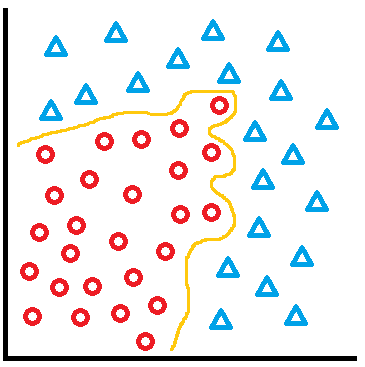
\includegraphics[scale=0.6]{figure1.png}
		\caption{Example of Logistic Regression Problem with 2 Features}
	\end{figure}
	%%%%%%%% FIGURE 1 %%%%%%%%
	
	However, if we have lots of features, we'll need to come up with hypothesis that include all of these features.
	
	With too many features, it might lead to overfitting problem and it can also be computationally expensive. Because of that, we'll need a new machine learning algorithm (Neural networks).
	
	%%%%%%%% Model Representation %%%%%%%%
	\section*{Model Representation}
	Neural networks was developed to simulate the networks of neurons in the brain. Some components in neural network include:
	\begin{itemize}
		\item Input wiress
		\item Output wires
	\end{itemize}

	\underline{Neuron model: logistic unit:}
	
	%%%%%%%% FIGURE 2 %%%%%%%%%
	\begin{center}
		\tikzstyle{line} = [draw, -latex']
		\tikzstyle{vertex} = [draw, circle,fill=white!100, node distance=1.55em, minimum height=2em]
		\tikzstyle{inv_vertex} = [draw=none, circle,fill=white!100, node distance=1.5em, minimum height=0.5em]
		\tikzstyle{description} = [draw=none, rectangle,fill=white!100, node distance=2.1em, minimum height=1em]
		
		\begin{tikzpicture}[node distance = 2.1em, auto]
		% Place nodes
		\node [vertex] (x0) {$x_{0}$};
		\node [inv_vertex, below of=x0] (i0) {};
		\node [vertex, below of=i0] (x1) {$x_{1}$};
		\node [inv_vertex, below of=x1] (i1) {};
		\node [vertex, below of=i1] (x2) {$x_{2}$};
		\node [inv_vertex, below of=x2] (i2) {};
		\node [vertex, below of=i2] (x3) {$x_{3}$};
		\node [inv_vertex, below of=x3] (i3) {};
		\node [vertex, right of=i1, node distance=4em] (a0) {$a_{0}$};
		\node [description, right of=a0, node distance=8em] (h) {$h_\theta (x)=\frac{1}{1+e^{-\theta^{T}x}}$};
		\node [description, left of=x0, node distance=10em] (desc) {bias unit or bias neuron};
		
		% Draw edges
		\path [line] (x0) -- node {input wires} (a0);
		\path [line] (x1) -- (a0);
		\path [line] (x2) -- (a0);
		\path [line] (x3) -- (a0);
		\path [line] (a0) -- (h);
		\path [line] (desc) -- (x0);
		\end{tikzpicture}
		\captionof{figure}{An example of a neuron model}\label{labelname}
	\end{center}
	%%%%%%%% FIGURE 2 %%%%%%%%%
	
	The neuron in figure 2 is called an artificial neuron with a sigmoid activation function.
	
	\[\theta =
	\begin{bmatrix}
	\theta_{0} \\
	\theta_{1} \\
	\vdots \\
	\theta_{n}
	\end{bmatrix}
	\]
	
	The vector $\theta$ is called "parameters" or "weights"
	
	\underline{Neural network:}
	
\end{document}